\documentclass[12pt]{ociamthesis}  % default square logo 
%\documentclass[12pt,beltcrest]{ociamthesis} % use old belt crest logo
%\documentclass[12pt,shieldcrest]{ociamthesis} % use older shield crest logo

%load any additional packages
\usepackage{hyperref}
\usepackage{amssymb}
\usepackage{float}
\usepackage{amsmath}
\usepackage{longtable}
%\usepackage{listings} %code listing, memasukkan code
\usepackage{listings}
\usepackage{xcolor}
 
\definecolor{codegreen}{rgb}{0,0.6,0}
\definecolor{codegray}{rgb}{0.5,0.5,0.5}
\definecolor{codepurple}{rgb}{0.58,0,0.82}
\definecolor{backcolour}{rgb}{0.95,0.95,0.92}
 
\lstdefinestyle{mystyle}{
    backgroundcolor=\color{backcolour},   
    commentstyle=\color{codegreen},
    keywordstyle=\color{magenta},
    numberstyle=\tiny\color{codegray},
    stringstyle=\color{codepurple},
    basicstyle=\ttfamily\footnotesize,
    breakatwhitespace=false,         
    breaklines=true,                 
    captionpos=b,                    
    keepspaces=true,                 
    numbers=left,                    
    numbersep=5pt,                  
    showspaces=false,                
    showstringspaces=false,
    showtabs=false,                  
    tabsize=2
}
 
\lstset{style=mystyle}
%input macros (i.e. write your own macros file called mymacros.tex 
%and uncomment the next line)
%\include{mymacros}

\title{Perancangan Aplikasi Qeuangans)\\[3ex]\textit{logbook}     %your thesis title,
}   %note \\[1ex] is a line break in the title

\author{Faris Muhammad Ihsan\\1.18.4.099\\Syabriena Putri Veriane\\1.18.4.094}             %your name
\college{}  %your college

%\renewcommand{\submittedtext}{change the default text here if needed}
\degree{Applied Bachelor Program of Informatics Engineering}     %the degree
\degreedate{Bandung\\ 2019}         %the degree date

%end the preamble and start the document
\begin{document}

%this baselineskip gives sufficient line spacing for an examiner to easily
%markup the thesis with comments
\baselineskip=18pt plus1pt

%set the number of sectioning levels that get number and appear in the contents
\setcounter{secnumdepth}{3}
\setcounter{tocdepth}{3}


\maketitle                  % create a title page from the preamble info
%\include{section/acknowlegements}   % include an acknowledgements.tex file
%\include{section/abstract}          % include the abstract
\begin{dedication}
`Jika Kamu tidak dapat menahan lelahnya belajar, \\
Maka kamu harus sanggup menahan perihnya Kebodohan.'\\ 
~Imam Syafi'i~\\
\end{dedication}

\begin{romanpages}          % start roman page numbering
\tableofcontents            % generate and include a table of contents
%\listoffigures              % generate and include a list of figures
\end{romanpages}            % end roman page numbering

%now include the files of latex for each of the chapters etc
\chapter{Pertemuan 1}

\section{Issues \#1}
Pada \textit{issues \#1} (\textit{Hardcoded String}) \textit{Hardcoded string} sebenarnya bukan merupakan \textit{error}, namun hanya sebagai peringatan. Peringatan ini terjadi karena menyimpan \textit{hard code string} pada file \textit{layout}. 
\begin{verbatim}
 android:text="Tabungan anda"
\end{verbatim}
Pemecahan dari Hardcoded String tersebut adalah dengan menuliskan\textit{string} pada file terpisah yang telah disediakan yaitu String.XML. Penulisan \textit{Hardcode String} yang terpisah pada file String.XML ini dapat memudahkan developer pada saat akan melakukan pengubahan nama. Developer hanya perlu mengubah pada file String.XML.

Solusinya, Pada file String.XML dituliskan baris kode seperti:
\begin{verbatim}
<resources>
<string name="app_name">Qeuangans</string>
<string name="Tabungan_anda">Tabungan Anda</string>
</resources>
\end{verbatim}

Kemudian, untuk Memanggil \textit{Hardcoded String} mengunakan perintah:
\begin{verbatim}
android:text="@string/Tabungan_anda
\end{verbatim}
Perintah tersebut dituliskan pada MainActivity.XML

\section{Issues \#2}
Pada \textit{issues \#2} (\textit{Error: Tag start is Not Closed}) berisi \textit{Error} pada file XML. Masalah ini disebabkan karena pada file XML tersebut terdapat baris perintah tanpa \textit{tag} penutup. XML merupakan file (\textit{eXtensible Markup Language}) dan merupakan bahasa \textit{Markup} layaknya bahasa HTML. Pada bahasa XML ini diperlukan tag pembuka dan penutup(contoh: </>), jika ada salah satu tag (baik pembuka maupun penutup) yang tidak ditulis, maka akan terbentuk error dan baris perintah tidak akan di eksekusi.
\begin{verbatim}
<TextView android:layout_width="wrap_content"
android:layout_height="wrap_content"
android:layout_alignParentTop="true"
android:layout_marginTop="18dp"
android:textColor="#000000"
app:layout_constraintBottom_toBottomOf="parent"
app:layout_constraintLeft_toLeftOf="parent"
app:layout_constraintRight_toRightOf="parent"
app:layout_constraintTop_toTopOf="parent"
android:text="@string/Tabungan_anda" 
\end{verbatim}

Pada \textit{error} ini memperbaikinya dengan cara menambahkan tag pada akhir baris perintah.
\begin{verbatim}
<TextView android:layout_width="wrap_content"
android:layout_height="wrap_content"
android:layout_alignParentTop="true"
android:layout_marginTop="18dp"
android:textColor="#000000"
app:layout_constraintBottom_toBottomOf="parent"
app:layout_constraintLeft_toLeftOf="parent"
app:layout_constraintRight_toRightOf="parent"
app:layout_constraintTop_toTopOf="parent"
android:text="@string/Tabungan_anda" />
\end{verbatim}

\section{Issues \#3}
Pada \textit{issues \#3} (\textit{Unusend Import Statement}) yaitu ketika kita akan mengimport suatu \textit{statement} maka akan menuliskannya pada awal baris kode. Mengimport disini berarti mengambil method yang ada pada kelas lain. Namun, \textit{Unused Import Statement} akan muncul ketika ada baris \textit{import} yang tidak digunakan. Hal ini hanya berupa peringatan dan bukan error.
\begin{verbatim}
package com.example.qeuangans;

import androidx.appcompat.app.AppCompatActivity;

import android.database.Cursor;
import android.graphics.Color;
import android.graphics.drawable.ColorDrawable;
import android.os.Bundle;
import android.util.Log;
import android.view.View; //Unused Import Statement: Issues \#6
import android.widget.AdapterView; //Unused Import Statement: Issues \#6
import android.widget.ArrayAdapter;
import android.widget.Toast;
\end{verbatim}

Solusinya adalah dengan menghapus import yang tidak digunakan karena methodnya tidak dibuat, maka perintah import tersebut dihapus. 
\begin{verbatim}
package com.example.qeuangans;

import androidx.appcompat.app.AppCompatActivity;

import android.database.Cursor;
import android.graphics.Color;
import android.graphics.drawable.ColorDrawable;
import android.os.Bundle;
import android.util.Log;
import android.widget.ArrayAdapter;
import android.widget.Toast;
\end{verbatim}

\section{Issues \#4}
Pada \textit{issues \#4} (\textit{Error: Cannot Resolve Method}) disini merupakan jenis \textit{error} yang disebabkan karena pemanggilan method yang salah atau method yang belum dibuat. Namun ketika baris kode ini dijalankan tidak ada nama method yang sesuai. Pada kasus ini, terdapat method yang belum dibuat namun sudah dipanggil. Kode Untuk memanggilnya menggunakan.
\begin{verbatim}
jmlSaldo();
\end{verbatim}
Pada pemanggilan tersebut terdapat method yang belum dibuat.

Solusi yang harus dilakukan adalah dengan menambahkan method dengan nama jmlSaldo(); beserta isi dari method yang dipanggil tersebut.
\begin{verbatim}
private void jmlSaldo() {
        Cursor cursor = db.saldo();
        while (cursor.moveToNext()) {
        textsaldo.append("Rp " + cursor.getString(0) + ",00");
        }
}
\end{verbatim}

\section{Issues \#5}
Pada \textit{issues \#5} (\textit{Error: Cannot Resolve Symbol}) Merupakan jenis error ketika ada objek yang dipanggil namun id nya tidak sama atau tidak ada (\textit{typo}), yang membuat baris kode tersebut tidak terbaca dan error sehingga objek untuk menampilkan saldo pada tampilah aplikasi tidak akan muncul.
\begin{verbatim}
<TextView
android:layout_width="match_parent"
android:layout_height="57dp"
android:layout_alignParentTop="true"
android:layout_marginTop="58dp"
android:hint="@string/Rp00"
android:textColor="#000000"
android:textSize="20sp" 
android:id="@+id/textado" <!-- Cannot Resolve Symbol: Issues #3--> />
\end{verbatim}

Solusinya adalah memberi id sesuai dengan yang dipanggil sehingga tampilan saldo akan muncul.
\begin{verbatim}
<TextView
        android:layout_width="match_parent"
        android:layout_height="57dp"
        android:layout_alignParentTop="true"
        android:layout_marginTop="58dp"
        android:hint="@string/Rp00"
        android:textColor="#000000"
        android:textSize="20sp" 
        android:id="@+id/textsaldo" <!-- Cannot Resolve Symbol: Issues #3--> />
\end{verbatim}

\section{Issues \#6}
Pada \textit{issues \#6} (\textit{intent Pindah()}) ini digunakan sebagai perintah untuk pindah dari \textit{Activity} yang satu ke yang lainnya. Intent merupakan objek yang menyediakan fungsi untuk pindah dari satu \textit{activity} ke \textit{activity} lainnya. Penggunaan intent dari \textit{method} pindah sebagai berikut:
\begin{verbatim}
public void Pindah(View view) {
        Intent intent = new Intent(MainActivity.this, InputData.class);
        startActivity(intent);
    }
\end{verbatim}
Intent pada method ini digunakan untuk pindah dari \textit{Activity} MainActivity.class ke \textit{Activity} InputData.class. Intent disini diaktifkan dengan perintah startActivity(intent); 

\section{Issues \#7}
Pada \textit{issues \#7} (\textit{Error: Semicolon Expected}) \textit{Semicolon Expected} adalah \textit{error} yang terjadi ketika sebuah baris program yang sudah ditulis kekurangan tanda \textit{semicolon}(;) pada akhir dari program, sehingga ketika baris program di eksekusi akan memunculkan peringatan \textit{error Semicolon Expected}. Contoh error:
\begin{verbatim}
startActivity(intent)
\end{verbatim}
Solusinya adalah dengan menambahkan \textit{semicolon}(;) pada akhir baris program.
\begin{verbatim}
startActivity(intent);
\end{verbatim}

\section{Issues \#8}
Pada \textit{issues \#8} (\textit{Error: Cannot resolve symbol}) \textit{Cannot Resolve Symbol} disini adalah ketika sebuah method yang menggunakan method dari kelas lainnya tapi tidak melakukan impor method maka akan muncul error ini. Solusinya adalah dengan cara menambahkan import method pada awal kode program.

\section{Issues \#9}
Pada \textit{issues \#9} (\textit{Error: \} Expected}) merupakan error yang disebabkan karena kurangnya tanda (\}) pada akhir kode program. Sama halnya seperti file XML yang memmerlukan tag pembuka dan penutup, sebuah method pada java juga harus menggunakan tanda pembuka(\{) dan tanda penutupnya(\}). Contoh \textit{Error: \} Expected}:
\begin{verbatim}
public void Pindah(View view) {
        Intent intent = new Intent(MainActivity.this, InputData.class);
        startActivity(intent);
\end{verbatim}
Solusinya adalah dengan menambahkan tanda penutup\} pada akhir method
\begin{verbatim}
public void Pindah(View view) {
        Intent intent = new Intent(MainActivity.this, InputData.class);
        startActivity(intent);
}
\end{verbatim}

\section{Issues \#10}
Pada \textit{issues \#10} (\textit{Error: Missing Parent}) \textit{Missing Parent} adalah \textit{error} yang disebabkan ketika kita ingin mendefinisikan objek namun belum mengimport library nya.
\chapter{Pertemuan 2}

\section{Issues \#11}
Pada \textit{issues \#11} (\textit{Cek mainActivity}) \textit{mainActivity} Merupakan activity yang utama ketika program dijalankan. Pada saat cek mainActivity, Program sudah bisa berjalan tanpa error. 
\begin{figure}[]
        \centering
        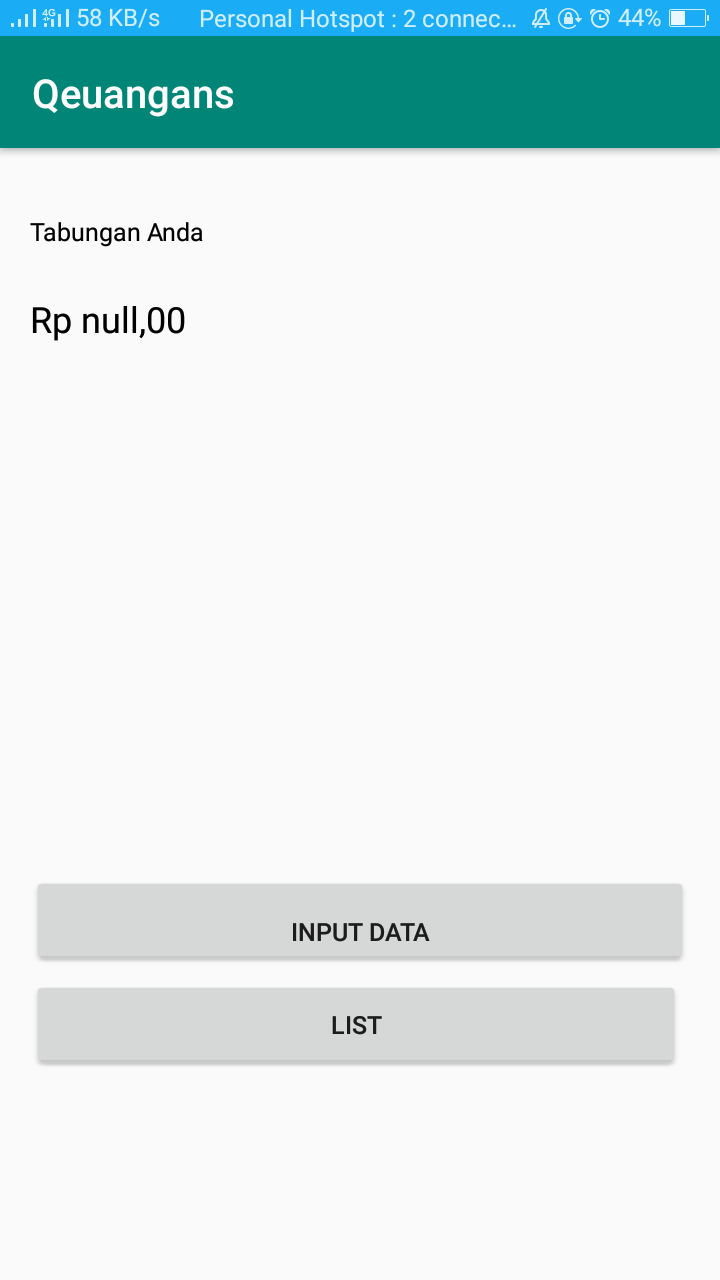
\includegraphics[scale = 0.3]{pictures/mainActivity.png}
        \caption{Gambar tampilan mainActivity}
        \label{mainActivity}
\end{figure}

\section{Issues \#12}
Pada \textit{issues \#12} (Penambahan Fitur Laporan) merupakan penambahan laporan.java pada aplikasi, penambahan fitur laporan ini menggunakan arraylist
\begin{verbatim}

        import androidx.appcompat.app.AppCompatActivity;

        import android.database.Cursor;
        import android.os.Bundle;
        import android.widget.ArrayAdapter;
        import android.widget.ListView;
        import android.widget.Toast;
        
        import java.util.ArrayList;
        
        public class laporan extends AppCompatActivity {
        
            DatabaseHelper db;
            ListView listLaporanK;
        
            @Override
            protected void onCreate(Bundle savedInstanceState) {
                super.onCreate(savedInstanceState);
                setContentView(R.layout.activity_laporan);
        
                listLaporanK = findViewById(R.id.listLaporanK);
        
                LK = new ArrayList<>();
        
                db = new DatabaseHelper(this);
        
                datalaporankeluar();
            }
        
            private void datalaporankeluar() {
                Cursor cursor = db.datalaporankeluar();
                if (cursor.getCount() == 0) {
                    Toast.makeText(this, "TIDAK ADA DATA", Toast.LENGTH_SHORT).show();
                } else {
                    while (cursor.moveToNext()) {
                        LK.add("\n" + cursor.getString(0) + "\n" + "Tanggal : " + cursor.getString(5) + "\n" + "\n" + "Pemasukan : " + cursor.getString(1)
                                + "\n" + "Jumlah : Rp " + cursor.getString(2) + ",00" + "\n" + "\n" + "Pengeluaran : " + cursor.getString(3)
                                + "\n" + "Jumlah : Rp" + cursor.getString(4) + ",00" + "\n");
                    }
                }
            }
        }
\end{verbatim}

\section{Issues \#13}
Pada \textit{issues \#13} (Tombol laporan tidak muncul pada aplikasi). Pada issues ini, tombol laporan tidak muncul pada aplikasi karena tombol tersebut belum dipanggil untuk dimunculkan. untuk memanggilnya menggunakan \begin{verbatim}
tombolLaporan = findViewById(R.id.tombolLaporan);
\end{verbatim}
disini berarti tombolLaporan ini dihubungkan dengan id dari tombol yang ada di mainActivity.XML dengan id tombolLaporan.

\section{Issues \#14}
Pada \textit{issues \#14} (\textit{Error: Undefined Method}) \textit{Undefined Method} merupakan jenis \textit{error} yang disebaban karena ketika method dipanggil tetapi method yang dipanggil tidak ada, maka akan muncul \textit{Undefined Method}. Solusi yang digunakan adalah dengan membuat method yang dipanggil.\\
Pemanggilan method:
\begin{verbatim}
Laporan();
\end{verbatim}
Method yang dipanggil:
\begin{verbatim}
public void Laporan(View view) {
    Intent intent = new Intent(MainActivity.this, laporan.class);
    startActivity(intent);
}
\end{verbatim}


\section{Issues \#15}
Pada \textit{issues \#15} (\textit{Error: ID is not Defined Anywhere}) \textit{ID is not Defined Anywhere} merupakan sebuah \textit{error}. \textit{Error} ini terjadi ketika sebuah id tombol pada activity\_main.XML ( android:id="Laporan") tidak memiliki ID yang benar, maka solusinya adalah memberikan id yang benar dengan menambahkan @+id pada awal kata "Laporan" contoh:
\begin{verbatim}
android:id="@+id/tombolLaporan"
\end{verbatim}
penggunaan @+id disini agar sesuai dengan penulisan yang digunakan pada android. 

\section{Issues \#16}
Pada \textit{issues \#16} (\textit{Error: Missing Constraints}) \textit{Missing Constraints} adalah \textit{error} yang terjadi ketika sebuah tampilan yang ada tidak ditentukan posisinya secara pasti. Contoh tampilan tanpa cnstraint pada activity\_main.XML: 
\begin{verbatim}
<TextView android:layout_width="wrap_content"
android:layout_height="wrap_content"
android:layout_alignParentTop="true"
android:layout_marginTop="18dp"
android:textColor="#000000"
android:text="@string/Tabungan_anda" 
\end{verbatim}
Jika posisi tidak ditentukan, maka yang terjadi adalah, tampilan tersebut akan otomatis berada pada (0,0) bagian layar atau di posisi kiri atas ketika aplikasi dijalankan. Solusi error tersebut adalah dengan menentukan posisinya. 
\begin{verbatim}
<TextView android:layout_width="wrap_content"
android:layout_height="wrap_content"
android:layout_alignParentTop="true"
android:layout_marginTop="18dp"
android:textColor="#000000"
android:text="@string/Tabungan_anda"
app:layout_constraintTop_toBottomOf="@+id/TombolLaporankeluar"
\end{verbatim}
layout\_constraintTop\_toBottomOf merupakan penentuan posisi pada bagian bawah yang dihubungkan dengan tampilan yang memiliki id "TombolLaporankeluar" yang ada pada activity\_main.XML.


\section{Issues \#17}
Pada \textit{issues \#17} (\textit{Error: Cannot Resolve Method add(java.lang.string)}) \textit{Cannot Resolve Method add(java.lang.string} adalah ketika method tidak bisa menambahkan value string pada arraylist yang akan ditampilkan. 

\section{Issues \#18}
Pada \textit{issues \#18} (Mengkoneksikan Database) Untuk mengkoneksikan database dapat menggunakan perintah:
\begin{verbatim}
db = new DatabaseHelper(this); 
\end{verbatim}
Perintah ini dimasukan pada file MainActivity.java

\section{Issues \#19}
Pada \textit{issues \#19} (\textit{Error: Cannot return value from void method.}) \textit{Error: Cannot return value from void method} merupakan sebuah \textit{error} yang disebabkan karena mencoba menggunakan perintah return(mengembalikan nilai) pada method void. Contoh pada DatabaseHelper.java:
\begin{verbatim}
public void datalaporankeluar(){ 
        SQLiteDatabase db = this.getReadableDatabase();
        Cursor saldo;
        saldo = db.rawQuery("SELECT SUM(" +COL3+")-SUM(" +COL5+") FROM "+TBLNAME, null);
        return saldo;
    }
\end{verbatim}
Sedangkan void sendiri merukpakan method yang tidak mengembalikan nilai sehingga return tidak bisa digunakan pada method void. Untuk solusinya yaitu dengan membuat methud tersebut menjadi function. Contoh: 
\begin{verbatim}
public Cursor datalaporankeluar(){ // Cannot return value from void method.  // Solusi ERROR 18. Issues #20 //
    SQLiteDatabase db = this.getReadableDatabase();
    Cursor saldo;
    saldo = db.rawQuery("SELECT SUM(" +COL3+")-SUM(" +COL5+") FROM "+TBLNAME, null);
    return saldo;
}
\end{verbatim}
Void disini diubah menjadi "cursor" karena digunakan untuk menganmbil value suatu data pada database yang di eksekusi dengan perintah "return saldo;"

\section{Issues \#20}
Pada \textit{issues \#20} (Koneksi ke Database) Untuk membuat koneksi ke database mengunakan perintah:
\begin{verbatim}
db = new DatabaseHelper(this);
\end{verbatim}
\chapter{Pertemuan 2}


%Belum Dikerjakan 
\section{Issues \#21}
Pada \textit{issues \#21} (\textit{Error: Cannot Resolve Symbol}) \textit{Cannot Resolve symbol} 

\section{Issues \#22}
Pada \textit{issues \#22} (Test Notifikasi) issues ini berisi test dari notifikasi yang sudah berjalan. Notifikasi ini menggunakan method Notiftest yang diletakan pada mainActivity.java.
\begin{verbatim}
public void Notiftest(View view) {
NotificationCompat.Builder builder = new NotificationCompat.Builder(this)
        .setSmallIcon(R.mipmap.ic_launcher)
           .setContentTitle("Issues Notif")
        .setAutoCancel(true)
        .setContentText("Berhasil Pak");
    NotificationManager notificationManager = 
    (NotificationManager)getSystemService(Context.NOTIFICATION_SERVICE);
    notificationManager.notify(NOTIFICATION_ID,builder.build());
}
\end{verbatim}

\section{Issues \#23}
Pada \textit{issues \#23} (Membuat layout pemasukan dan pengeluaran)layout dibuat dalam file xml dengan memasukan tombol-tombol dan inputan text. Dalam pembuatan layout ini menggunakan cara \textit{Drag and Drop} melalui opsi yang sudah disediakan oleh android studio dan menghasilkan tampilan seprti: 
\begin{figure}
    \centering
    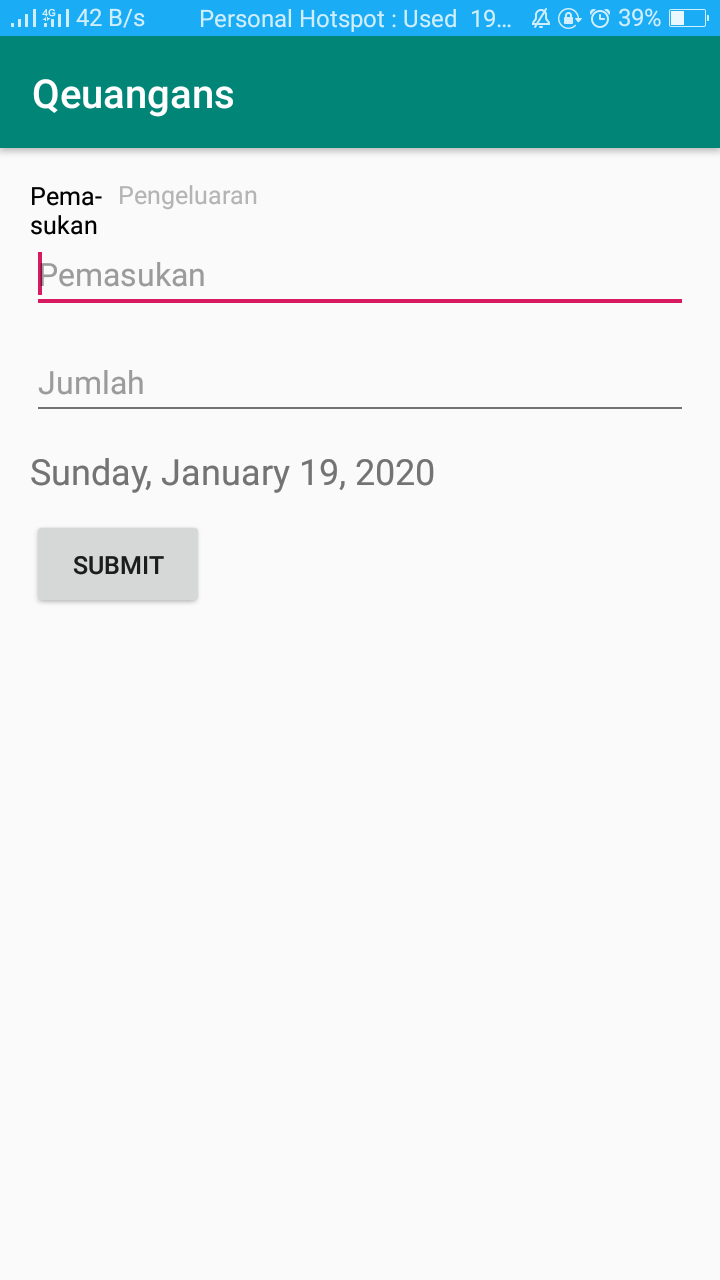
\includegraphics[scale = 0.3]{pictures/pemasukan_layout.png}
    \caption{Gambar Layout Pemasukan}
\end{figure}
\begin{figure}
    \centering
    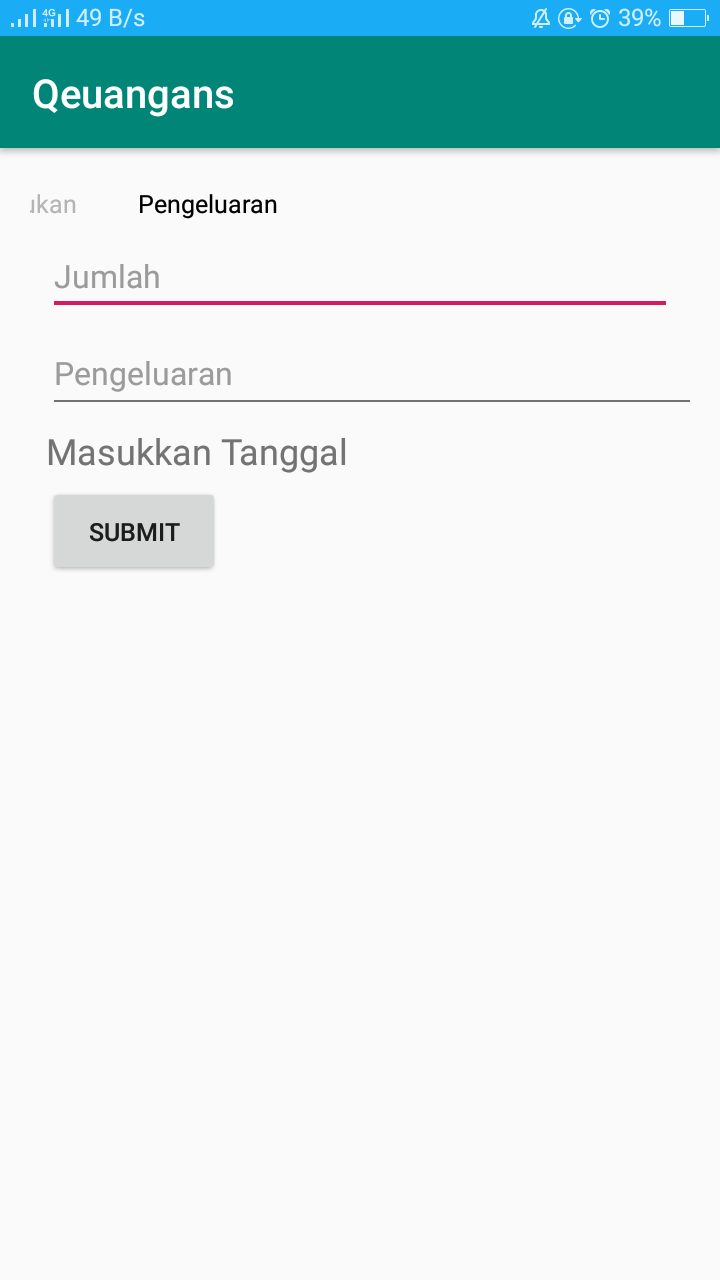
\includegraphics[scale = 0.3]{pictures/pengeluaran_layout.png}
    \caption{Gambar Layout Pengeluaran}
\end{figure}

\section{Issues \#24}
Pada \textit{issues \#24} (\textit{Datepicker Dialog} pada input pengeluaran). \textit{Datepicker} merupakan fasilitas yang disediakan android untuk memilih tanggal. Untuk menggunakan \textit{datepicker} menggunakan baris kode seperti berikut:
\begin{verbatim}
final int year = calendar.get(Calendar.YEAR);
final int month = calendar.get(Calendar.MONTH);
final int day = calendar.get(Calendar.DAY_OF_MONTH);

tglpengeluaran.setOnClickListener(new View.OnClickListener() {
    @Override
    public void onClick(View view) {
        DatePickerDialog datepickerdialog = 
        new DatePickerDialog(InputData2.this,
                android.R.style.Theme_Holo_Light_Dialog_MinWidth,
                setListener, year,month,day);
        datepickerdialog.getWindow().setBackgroundDrawable
        (new ColorDrawable(Color.TRANSPARENT));
        datepickerdialog.show();
    }
});
setListener = new DatePickerDialog.OnDateSetListener() {
    @Override
    public void onDateSet(DatePicker datePicker, int year, int month, 
    int dayOfMont) {
        month = month+1;
        String date = day+"/"+month+"/"+year;
        tglpengeluaran.setText(date);
    }
};
\end{verbatim}


\section{Issues \#25}
Pada \textit{issues \#25} Menambahkan getar pada notifikasi. Bars kode ini dimasukan pada method notiftest pada mainActivity.java
\begin{verbatim}
    .setContentText("Berhasil Pak");
\end{verbatim}

\section{Issues \#26}
Pada \textit{issues \#26} Menambahkan \textit{DatePickerDialog} pada InputData.java
\begin{verbatim}
    tglpemasukan.setOnClickListener(new View.OnClickListener() {
            @Override
            public void onClick(View view) {
                DatePickerDialog datePickerDialog = new DatePickerDialog(
                        InputData.this,android.R.style
                        .Theme_Holo_Light_Dialog_MinWidth,
                        setListener,year,month,day);
                datePickerDialog.getWindow().setBackgroundDrawable
                (new ColorDrawable(Color.TRANSPARENT));
                datePickerDialog.show();
            }
        });

        setListener = new DatePickerDialog.OnDateSetListener() {
            @Override
            public void onDateSet(DatePicker datePicker, int year,
            int month, int dayOfMonth) {
                month = month+1;
                String date = day+"/"+month+"/"+year;
                tglpemasukan.setText(date);
            }
        };
\end{verbatim}


\section{Issues \#27}
Pada \textit{issues \#27} menambahkan suara pada notifikasi dengan memasukan 
\begin{verbatim}
    .setSound(RingtoneManager.getDefaultUri
    (RingtoneManager.TYPE_NOTIFICATION));
\end{verbatim}
pada Notiftest() pada mainActivity.java

\section{Issues \#28}
Pada \textit{issues \#28} (Mengubah fungsi Pada Pemasukan). Pengubahan fungsi ini dilakukan pada InputData.java karena layout pemasukan dan pengeluaran yang dibagi menjadi dua.

\section{Issues \#29} 
Pada \textit{issues \#29} (\textit{Error: Cannot Resolve Symbol 'jenispengeluaran'})
\begin{verbatim}
private void AddData() {
    inputmasuk.setOnClickListener(
            new View.OnClickListener() {
                @Override
                public void onClick(View view) {
                        boolean isInseted = myDB.insertData
                        (jenispemasukan.getText().toString(),
                                jmlpemasukan.getText().toString(), 
                                **jenispengeluaran** .getText().toString(),
                                jmlpengeluaran .getText().toString(), 
                                tglpemasukan.getText().toString());
                        if (isInseted = true)
                            Toast.makeText(InputData.this, "INPUT BERHASIL", 
                            Toast.LENGTH_LONG).show();
                        else
                            Toast.makeText(InputData.this, "INPUT GAGAL", 
                            Toast.LENGTH_LONG).show();

                }
            }
\end{verbatim}
Error ini terjadi karena method \textit{insertData} pada \textit{DatabaseHelper.java} tidak ada perintah untuk melakukan inputan jenispengeluaran sehingga pada method AddData() diatas terjadi \textit{error cannot resolve symbol}. Solusinya adalah dengan menghapus jenispengeluaran pada method AddData.
\begin{verbatim}
private void AddData() {
    inputmasuk.setOnClickListener(
            new View.OnClickListener() {
                @Override
                public void onClick(View view) {
                        boolean isInseted = myDB.insertData(jenispemasukan
                        .getText().toString(),
                                jmlpemasukan.getText().toString(), tglpemasukan
                                .getText().toString());
                        if (isInseted = true)
                            Toast.makeText(InputData.this, "INPUT BERHASIL", 
                            Toast.LENGTH_LONG).show();
                        else
                            Toast.makeText(InputData.this, "INPUT GAGAL", 
                            Toast.LENGTH_LONG).show();

                }
            }
\end{verbatim}

\section{Issues \#30}
Pada \textit{issues \#30} (Menambahkan \textit{Current Date} pada Input Pemasukan (InputData.java)). Current Date disini merupakan tanggal pada hari ini, cara menambahkannya dengan menambahkan baris perintah
\begin{verbatim}
Calendar calendar = Calendar.getInstance();
String currentDate = DateFormat.getDateInstance(DateFormat.FULL)
.format(calendar.getTime());
\end{verbatim}
pada InputData.java

\section{Issues \#31}
Pada \textit{issues \#31}

\section{Issues \#32}
Pada \textit{issues \#32}

\section{Issues \#33}
Pada \textit{issues \#33}

\section{Issues \#34}
Pada \textit{issues \#34}

\section{Issues \#35}
Pada \textit{issues \#35}

\section{Issues \#36}
Pada \textit{issues \#36}

\section{Issues \#37}
Pada \textit{issues \#37}

\section{Issues \#38}
Pada \textit{issues \#38}

\section{Issues \#39}
Pada \textit{issues \#39}

\section{Issues \#40}
Pada \textit{issues \#40}
\section{Issues \#41}
Pada \textit{issues \#41}

\section{Issues \#42}
Pada \textit{issues \#42}

\section{Issues \#43}
Pada \textit{issues \#43}

\section{Issues \#44}
Pada \textit{issues \#44}

\section{Issues \#45}
Pada \textit{issues \#45}

\section{Issues \#46}
Pada \textit{issues \#46}

\section{Issues \#47}
Pada \textit{issues \#47}

\section{Issues \#48}
Pada \textit{issues \#48}

\section{Issues \#49}
Pada \textit{issues \#49}

\section{Issues \#50}
Pada \textit{issues \#50}
\include{section/chapter6}
\include{section/chapter7}
\include{section/chapter8}
%next line adds the Bibliography to the contents page
%\addcontentsline{toc}{chapter}{Bibliography}
%uncomment next line to change bibliography name to references
%\renewcommand{\bibname}{References}
%\bibliography{references}        %use a bibtex bibliography file refs.bib
%\bibliographystyle{plain}  %use the plain bibliography style

\end{document}

